\documentclass{sigchi}

% Use this command to override the default ACM copyright statement (e.g. for preprints). 
% Consult the conference website for the camera-ready copyright statement.


%% EXAMPLE BEGIN -- HOW TO OVERRIDE THE DEFAULT COPYRIGHT STRIP -- (July 22, 2013 - Paul Baumann)
% \toappear{Permission to make digital or hard copies of all or part of this work for personal or classroom use is 	granted without fee provided that copies are not made or distributed for profit or commercial advantage and that copies bear this notice and the full citation on the first page. Copyrights for components of this work owned by others than ACM must be honored. Abstracting with credit is permitted. To copy otherwise, or republish, to post on servers or to redistribute to lists, requires prior specific permission and/or a fee. Request permissions from permissions@acm.org. \\
% {\emph{CHI'14}}, April 26--May 1, 2014, Toronto, Canada. \\
% Copyright \copyright~2014 ACM ISBN/14/04...\$15.00. \\
% DOI string from ACM form confirmation}
%% EXAMPLE END -- HOW TO OVERRIDE THE DEFAULT COPYRIGHT STRIP -- (July 22, 2013 - Paul Baumann)

\toappear{Submitted to CHI2014. Do not cite or distribute.}

% Arabic page numbers for submission. 
% Remove this line to eliminate page numbers for the camera ready copy
\pagenumbering{arabic}


% Load basic packages
\usepackage{balance}  % to better equalize the last page
\usepackage{graphics} % for EPS, load graphicx instead
\usepackage{times}    % comment if you want LaTeX's default font
\usepackage{url}      % llt: nicely formatted URLs
\usepackage{gensymb}
\usepackage{afterpage}
% see http://tex.stackexchange.com/questions/46055/typesetting-with-inch-symbols-and-sizes-in-inches
\usepackage{mathpazo,amsmath}
\def\inch#1{#1''}
\def\ft#1{#1'\thinspace}

\usepackage{subcaption}

% llt: Define a global style for URLs, rather that the default one
\makeatletter
\def\url@leostyle{%
  \@ifundefined{selectfont}{\def\UrlFont{\sf}}{\def\UrlFont{\small\bf\ttfamily}}}
\makeatother
\urlstyle{leo}


% To make various LaTeX processors do the right thing with page size.
\def\pprw{8.5in}
\def\pprh{11in}
\special{papersize=\pprw,\pprh}
\setlength{\paperwidth}{\pprw}
\setlength{\paperheight}{\pprh}
\setlength{\pdfpagewidth}{\pprw}
\setlength{\pdfpageheight}{\pprh}

% Make sure hyperref comes last of your loaded packages, 
% to give it a fighting chance of not being over-written, 
% since its job is to redefine many LaTeX commands.
\usepackage[pdftex]{hyperref}
\hypersetup{
pdftitle={SIGCHI Conference Proceedings Format},
pdfauthor={LaTeX},
pdfkeywords={SIGCHI, proceedings, archival format},
bookmarksnumbered,
pdfstartview={FitH},
colorlinks,
citecolor=black,
filecolor=black,
linkcolor=black,
urlcolor=black,
breaklinks=true,
}

% create a shortcut to typeset table headings
\newcommand\tabhead[1]{\small\textbf{#1}}

%use these commands while writing
\newcommand {\bjoern}[1]{{\color{red}\bf{BH: #1}\normalfont}}
\newcommand {\ben}[1]{{\color{blue}\bf{BZ: #1}\normalfont}}
\newcommand {\sean}[1]{{\color{blue}\bf{SC: #1}\normalfont}}
\newcommand {\claire}[1]{{\color{blue}\bf{CT: #1}\normalfont}}
\newcommand {\studyquote}[1]{\em ``#1''\normalfont}
%comment out the above and uncomment these for final submit
%\newcommand {\bjoern}[1]{}
%\newcommand {\ben}[1]{}
%\newcommand {\sean}[1]{}
%\newcommand {\claire}[1]{}

% End of preamble. Here it comes the document.
\begin{document}

\title{GlasSees - Providing Context Menus for the Real World Through Head-Worn Infrared Targeting}

\numberofauthors{1}
\author{
 \alignauthor Anonymous for submission
%  \alignauthor 3rd Author Name\\
%    \affaddr{Affiliation}\\
%    \affaddr{Address}\\
%    \email{e-mail address}\\
%    \affaddr{Optional phone number}
}

\maketitle

\begin{abstract}
%!TEX root = uist14.tex

%% Yang suggests: Interacting with smart objects in the physical space efficiently is a realistic challenge as these objects become ubiquitous. In this paper, we contribute HOBS, a set of novel methods for selecting physical objects at a distance using infrared-sensed head orientations. We augment a commercial head-worn device, Google Glass, with an infrared (IR) emitter to select targets equipped with IR receivers. We present the iterative design process of our methods, involving a series of interaction technique and hardware design and user evaluations....
Emerging head-worn computing devices can enable interactions with smart objects in physical spaces.
%
We present the iterative design and evaluation of \systemname -- a Head-Orientation Based Selection technique for interacting with these devices at a distance. We augment a commercial wearable device, Google Glass, with an infrared (IR) emitter to select targets equipped with IR receivers. Our first design shows that a naive IR implementation can outperform list selection, but has poor performance when refinement between multiple targets is needed. A second design uses IR intensity measurement at targets to improve refinement. To address the lack of natural mapping of on-screen target lists to spatial target location, our third design infers a spatial data structure of the targets enabling a natural head-motion based disambiguation.
%
Finally, we demonstrate a universal remote control application using HOBS and report qualitative user impressions.

\end{abstract}

\keywords{
	smart devices; universal remote control; wearable computing; glass
}

\category{H.5.m.}{Information Interfaces and Presentation (e.g. HCI)}{Miscellaneous}

%$See: \url{http://www.acm.org/about/class/1998/}
%for more information and the full list of ACM classifiers
%and descriptors. 
%\textcolor{red}{Mandatory section to be included in your
%final version. On the submission page only the classifiers'
%letter-number combination will need to be entered.}

\section{Introduction}
Increasingly, devices and services in our built environment are networked and can be controlled remotely. The proliferation of smart, controllable devices such as intelligent lighting, AV equipment, HVAC systems, or kitchen appliances raises the question of how to best interact with them. 

Today, commercial solutions use handheld mobile devices as {\em universal remote controls} to control such appliances~\bjoern{refs!}. Commonly, users first browse a list of all available devices, and then call up a device-specific user interface. This method faces two challenges: {\em naming} and {\em scoping}. Assigning clear names is non-trivial. In shared spaces, the person trying to control the device might not be the one that named it - e.g., while an office building manager may know what ``Light 4 in area E'' corresponds to, an occupant may not. Second, without a method of scoping selection to automatically filter non-relevant devices, paging though long lists of names or navigating hierarchies becomes potentially more cumbersome than the physical action the ``convenient'' software solution was meant to replace.

To address these challenges, research has introduced techniques of augmenting mobile devices, e.g., with laser pointers, to enable direct aiming at target devices~\cite{beigl_point_1999,patel_2-way_2003}. While promising, some drawbacks of using handheld devices are that the device first has to be retrieved (e.g., from a pocket) and aimed; that two hands may be necessary for operation (one to hold the device, one to operate the touch screen); and that the user's visual attention is now split between looking down at a screen and out at the device to-be-controlled. 

\begin{figure}[t]
\centering
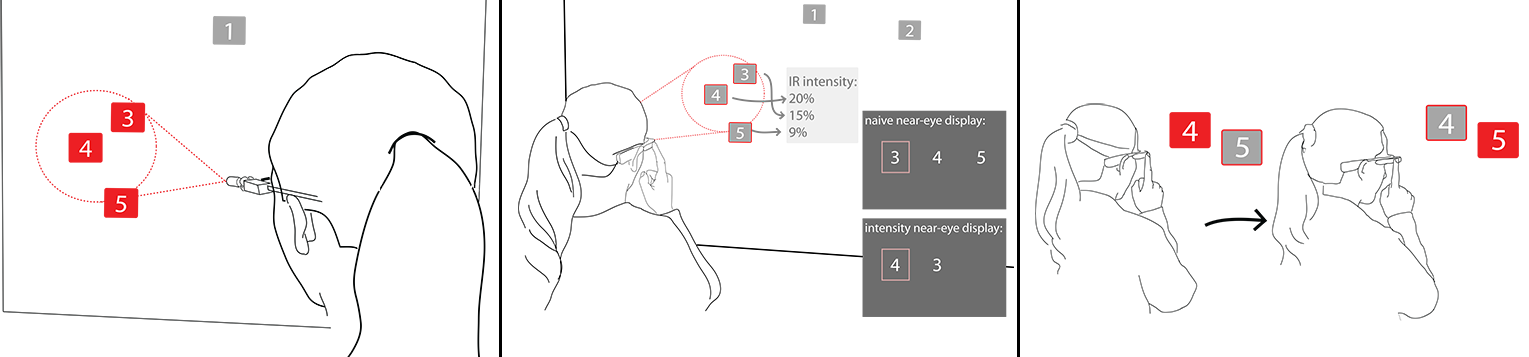
\includegraphics[width=1.0\columnwidth]{figures/teaser.png}
\caption{Teaser figure. Needs a caption.}
\label{fig:teaser}
\end{figure}

In this paper, we introduce a novel method for selecting and controlling smart appliances in physical spaces though the use of a head-worn computing device with near-eye display and wireless communication. We augment Google Glass\footnote{\url{http://www.google.com/glass/start/}} with custom hardware for this purpose. Users first look in the direction of the device they wish to control to initiate interaction (e.g., at a lamp to control lighting, or at a speaker to change music playback volume).  If multiple devices fall within communication range, an disambiguation technique that combines on-screen information as well as visual feedback on the target devices lets users select their desired target. Once acquired, a device specific control UI shown on the head-mounted display enables adjustment of discrete and continuous parameters through a touchpad interface (see Figure~\ref{fig:teaser}).

Our hardware relies on infrared communication between Glass and target devices to establish a connection; and on wireless 802.15.4 radio communication to exchange control messages.  Glass is augmented with a narrow-beam IR emitter and a 802.15.4 radio. Target devices similarly have IR receivers and radios. This combination enables users to initiate interaction by orienting their head; but once initiated, users are free to look away from the target device while issuing control commands.

While prior work has tended to focus on proofs-of-concept, we also contribute empirical data on the system performance, usability, and user experience of  head-orientation targeting and device control. We first report measurements of range and beam characteristics of our controller. We then conduct a study that compares acquisition times for physical targets in a room for our technique and an alternative list selection interface. We find that target acquisition through head orientation is preferred by users and is faster than list selection, given the constraints of linear input using a head-worn touch controller. We also report qualitative results from $n$ participants who use our system for home automation tasks.







%!TEX root = sui14.tex
\section{Background and Related Work}
Our approach is related to head- and eye-controlled interfaces, area cursors and prior work on hardware devices for pointing in physical spaces.

\vfill
\ben{make sure no section title appears at the end of any column.}
\subsection{Head and Gaze Input}
\changes{Head movement has long been used for virtual camera control in VR applications~\cite{pausch_user_1993} and as an assistive input technology for cursor control of desktop applications~\cite{radwin1990method}. However, it is notable that human neck muscles have a lower bandwidth than other muscle groups, e.g., the wrist~\cite{card_morphological_1991}.}
%
%Card, summarizing other work, shows that neck muscles are a poor muscle group for pointing in general: neck muscles only have a bandwidth of about $4.2bits/s$ (compared to $23bits/s$ of wrist muscles used by a standard mouse~\cite{Card:1991:MAD:123078.128726}. 
%
Prior work often focused on head orientation for controlling graphical interfaces; in contrast, we apply this modality to selection in physical spaces.

Gaze can also be used to control graphical user interfaces~\cite{kumar2007eyepoint}. While there are wearable gaze trackers~\cite{bulling2009wearable}, turning information about a concrete point in space where a user is looking into a selection requires a map with known target locations.
Our system works through point-to-point IR communication and does not require an {\em a priori} map or markers. Target objects in the environment can also be equipped with individual cameras that watch the user~\cite{smith2013gaze,vertegaal2005media}. Such an approach can enable similar benefits as our approach, but is computationally more expensive than our single-pixel sensor solution and may not work at greater distances or angles, because it relies on finding the user's pupils in a camera image.

%Our work is closer in spirit to Selker's headworn system~\cite{Selker:2001:EGE:634067.634176}.

\subsection{Area Cursors}
\changes{
In 2D area cursors for GUIs, the activation area of the cursor is enlarged, which facilitates acquiring smaller targets~\cite{kabbash1995prince}. We argue that head orientation pointing has analogous characteristics (limited pointing performance and accuracy). Area cursors are especially appropriate for individuals with motor control impairments or difficulties~\cite{worden1997making,findlater2010enhanced}. Similar ideas have also been extended into 3D to provide selection with progressive refinement in 3D scenes~
\cite{bacim2013design}. In all area and space cursors, the large activation area can lead to multiple targets being selected and disambiguation is needed. This paper describes the trade-offs between several disambiguation approaches.


%We conceptualize area pointing as a two-stage process: in the {\em coarse} phase, which we call {\em scanning}, users move so the activation area intersects with the target object (and possibly other, unintended targets). In the {\em refinement} phase, they adjust so only the intended target will be selected. Many disambiguation techniques are possible for refinement -- this paper describes the trade-offs between several of them.
}

\subsection{Pointing in Physical Spaces}
Rukzio ~\cite{rukzio_experimental_2006} studied alternative methods for selecting devices in physical spaces and found that users strongly preferred either tapping target appliances with a mobile device or pointing at a distance to browsing a list.

Several approaches to spatial selection with handheld devices~\cite{beigl_point_1999,patel_2-way_2003,wilson_xwand:_2003,schmidt_picontrol:_2012,kemp_point-and-click_2008} or finger-worn devices~\cite{merrill_augmenting_2007} exist. 
%and exchanging information with smart infrastructure sensor networks ~\cite{lifton_tricorder:_2007,mittal_ubicorder:_2011,costanza_sensortune:_2010}. 
In some techniques, users select objects of interest with laser pointers. The laser dot provides immediate visual feedback to the user about what is being selected; however, its small target area makes it poorly matched to head orientation input.
Other approaches rely on virtual room models in which a user's location is estimated using IMU-based orientation sensing~\cite{wilson_xwand:_2003,lifton_tricorder:_2007} -- in contrast, our technique does not require a static map ahead of time.
%Other targeting systems use IR with handheld pointers~\cite{swindells_that_2002} as well as wearable devices such as rings and Bluetooth audio earpieces~\cite{merrill_augmenting_2007} to connect to smart devices. 
Our system tackles an unresolved issue of prior approaches -- navigating an area dense with potential targets and resolving selection ambiguity.

\subsection{Vision- and Projection-Based Target Selection}
\changes{Many alternative solutions for detecting devices in contained spaces
rely on computer-vision recognition of printed tags on devices. Unfortunately,
these methods either impose significant constraints on the camera used for
detection~\cite{Bokode}, require large or obtrusive tags~\cite{Dataglyphs}, or
are designed to work specifically at short distances~\cite{CyberCode}. Passive
markers also cannot show visual feedback in the environment.  Handheld
projectors can both display a user interface in space and communicate control
information optically, e.g., by encoding information temporally (using Gray
codes in Picontrol~\cite{schmidt_picontrol:_2012} and RFIG
Lamps~\cite{raskar_rfig_2004}) or spatially (using QR codes in the infrared
spectrum in SideBySide~\cite{willis_sidebyside:_2011}). Our solution is similar
in spirit but requires only small, low-cost IR emitters and detectors.
\bjoern{need a stronger statement here}} \achal{Tried emphasizing the smaller
requirements, not sure what else we can say.}

%However, visible tags at appropriate sizes may be rejected by users because of their negative aesthetic effect on the space.

%\subsection{Markers and Vision Methods}
%\achal{Not sure where to put this, feel free to move.}
%
%\ben{For CV, I think related work is one option to go; however, the requirement of being related work is that -- we need to reference them. There are a few examples ``require large, obtrusive tags, and inevitably lack feedback from passive devices in the environment'' which should be referenced. That's why I am thinking of putting this to discussion.}
%


%\ben{Reviewers suggest considering computer vision-based techniques with markers in the environment (such as %QR codes, or Bokode [Mohan] which extends the working distance to a few meters for visual tags). We considered this direction and found several drawbacks, including computational complexity, low accuracy when targets are far, the absence of real-time environment feedback with passive tags, and aesthetic issues with QR codes. While we don't claim our choice of IR is optimal, it has important advantages -- it is low-cost, readily available and quite suitable for area selection. We can weaken our claim and add explanations of how disambiguation techniques might generalize to other methods of implementing target identification.}

%\achal{Read and discussed the Bokode paper and CV in general. Unsure about what
%to do regarding "weakening our claim."}


%\ben{new related works from reviewers}. \bjoern{folded in}
%\changes{RFIG Lamps and photosensing wireless tags [Raskar et al] use a projector and data is encoded in each pixel so that tags can localize themselves for target selection. Our IR emitter, a relatively low-cost solution, doesn’t have this feature but shares the commonality of covering an area for the ease of selection. At the end of their paper, they envision an IR-based system to solve ambient light problems. Our work lies in that direction and also contributes evaluations with user studies.
%Progressive Refinement [Bacima] studies several progressive refinement selection modalities, which is close to our two-stage selection; but our contexts are head-orientation as it reflects users' point of interest.
%}

%!TEX root = sui14.tex
\section{IR for head orientation-based targeting}
In this section, we present our hardware platform (IR targeting) and interaction model (head-orientation based) that we will use throughout our iterative designs.

\subsection{Hardware}
%A central hypothesis of this paper is that the area cursor paradigm~\cite{kabbash1995prince} is well matched to head orientation selection. Head orientation input is imprecise because it does not capture eye movement and has to rely on a low-bandwidth muscle group. Therefore, point selection techniques like laser pointers are not appropriate. 

We hypothesize that infrared (IR) emitters are a good technology match for head orientation selection, since they emit light within a given angle, resulting in a cone in front of the emitter where the light is visible. IR LEDs with many different beam angles are commercially available. We augment Google Glass with a 940nm 5mm IR emitter with $10^\circ$ beam angle (OSRAM SFH 4545). The emitter is controlled by an additional microcontroller which communicates with Google Glass through Bluetooth radio, since Glass does not directly support hardware modification (see Figure~\ref{fig:glass}). Target devices use Vishay TSOP38238 IR receivers. Data is encoded using standard IR remote protocols at 38.0kHz.

IR signals are used for initial line-of-sight targeting; subsequently, we use bidirectional wireless communication to send information such as target IDs and signal strength from targets back to Glass. We have chosen the commercial off-the-shelf ZigBee implementation (XBee based on 802.15.4 radio) for this purpose (see Figure~\ref{fig:architecture}). This architecture was mostly chosen for reasons of expediency and we do not claim optimality for prototyping decisions. Future head-mounted devices could clearly integrate IR emitters; other wireless techniques (WiFi, Bluetooth) can also be used.

% The IR emitter is the one from OSRAM Opto Semiconductors Inc with manufacturer part number SFH 4545. From the datasheet, it has a view angle of $10^\circ$. Part of the reason we have chosen it is because the radiant intensity can quite high if we provide it with sufficient current flow (550mW/sr @ 100mA). We can then easily adjust it using a resistor to satisfy different demands. 
% % transmitter webpage: http://www.digikey.com/product-search/en?x=0&y=0&lang=en&site=us&KeyWords=475-2919-ND
% For the IR receiver, we use 38.0kHz IR Receiver Modules from Vishay Semiconductor Opto Division (manufacturer part number TSOP38238). 
% % receiver webpage http://www.digikey.com/product-detail/en/TSOP38238/751-1227-ND/1681362
% In order to read the IR intensity, we integrates another IR light-to-voltage converter from AMS-TAOS USA Inc (manufacturer part number TSL267-LF) which is pretty sensitive to IR irradiance. 
% % http://www.digikey.com/product-detail/en/TSL267-LF/TSL267-LF-ND/3095052



%% \ben{no mention of target hardware yet. I have checked in an image of the targets ``targets.JPG'' in case we need.}

%For the IR receiver, we use 38.0kHz IR Receiver Modules from Vishay Semiconductor Opto Division (manufacturer part number TSOP38238). 
% receiver webpage http://www.digikey.com/product-detail/en/TSOP38238/751-1227-ND/1681362
%In order to read the IR intensity, we integrates another IR light-to-voltage converter from AMS-TAOS USA Inc (manufacturer part number TSL267-LF) which is pretty sensitive to IR irradiance. 
% % http://www.digikey.com/product-detail/en/TSL267-LF/TSL267-LF-ND/3095052

\begin{figure}[t]
\centering
\includegraphics[width=0.95\columnwidth]{figures/GlassWithArduino.jpg}
\caption{Our Glass hardware: Google Glass augmented with a repositionable IR holder, and an additional microcontroller that communicates with Google Glass and controls IR emitter.}
\label{fig:glass}
\end{figure}

\begin{figure}[t]
\centering
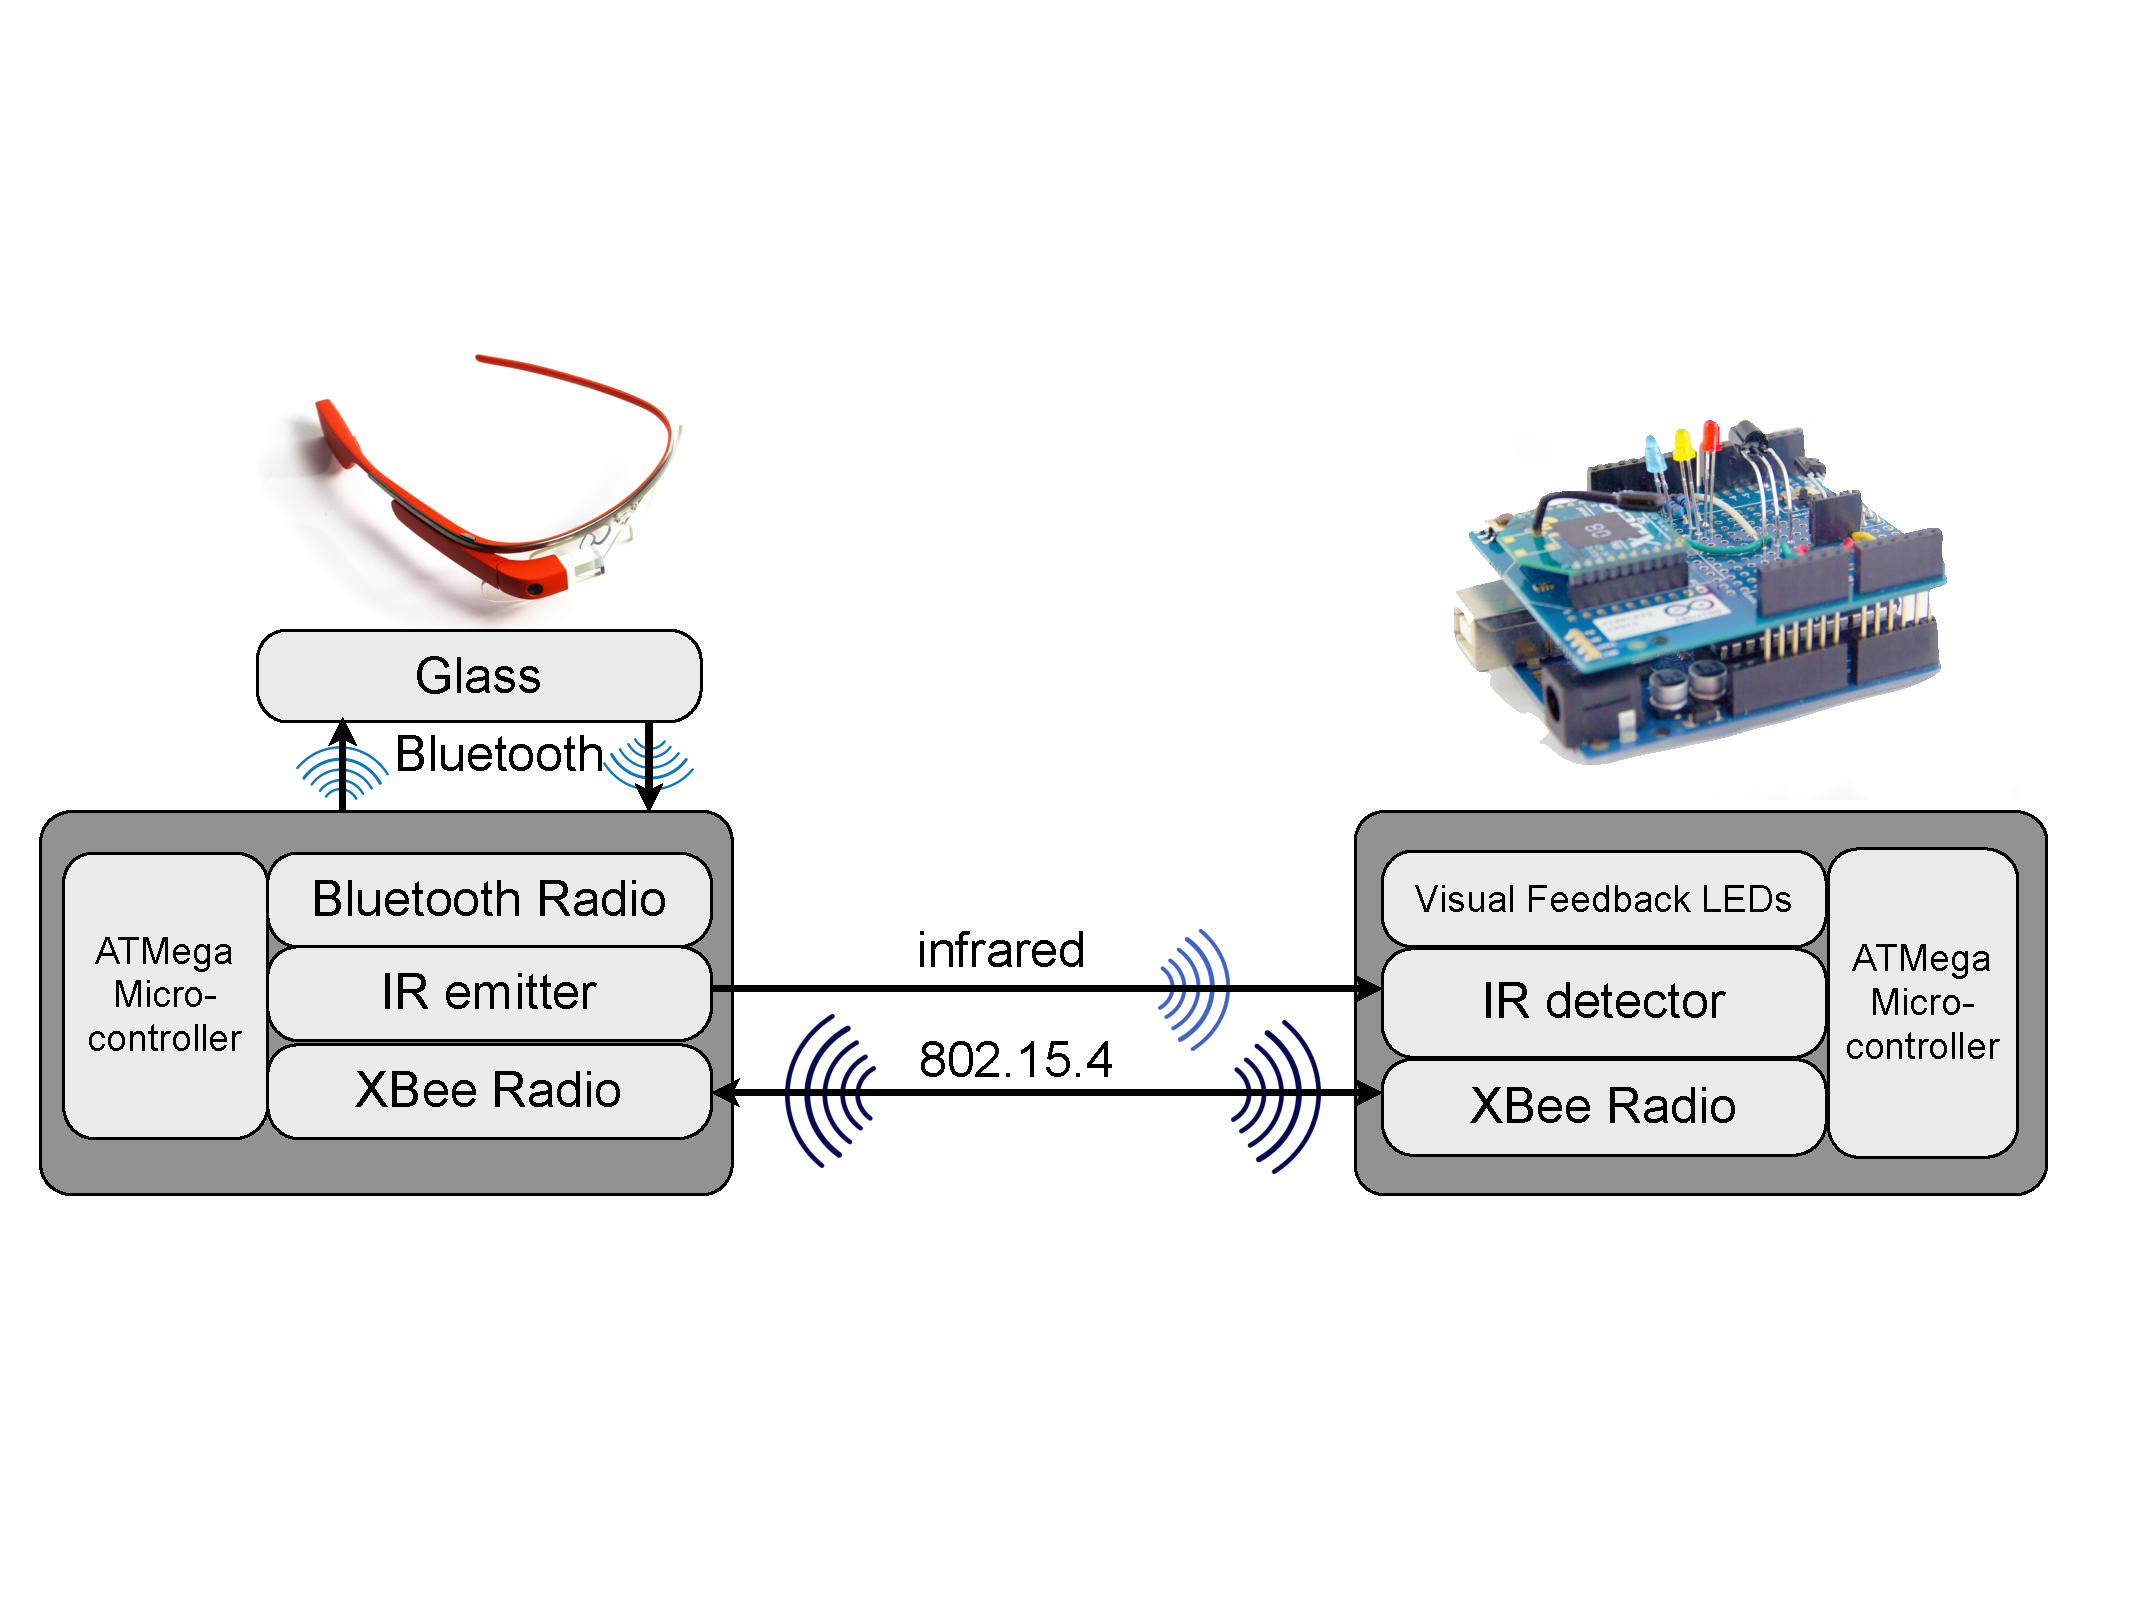
\includegraphics[width=0.95\columnwidth]{figures/architecture_new}
\caption{Our System architecture diagram. The selection is initiated through infrared but confirmed over 802.15.4.}
\label{fig:architecture}
\end{figure}

\newpage %bjoern hack fix
\subsection{Interaction Model}
From the user's perspective, interaction with \systemname proceeds in two stages (Figure~\ref{fig:interaction}): 


{\bf Scan:} The user first scans the environment to locate the position of the target. During this stage, Glass constantly sends out IR signals, and  targets offer immediate visual feedback when they receive a signal. The user confirms his desire to connect to a target by tapping on the Glass touchpad. Glass collects the responses from targets that have received IR reception through the backchannel of XBee. If there is only one single target in IR range, it is automatically selected. However, in a dense environment where multiple targets are within range, the user needs to refine his selection.


{\bf Refine:} When disambiguation is needed, the user must make an explicit selection among the targets within their view range. We have designed multiple refinement mechanisms -- all of which enable the user to select one from a subset of targets. The user confirms the current selection with a tap. Since the purpose of this stage is to disambiguate among potential targets, we will also use {\em disambiguation} to refer to this stage. Finally, a tap confirms a decision.


\begin{figure}[t!]
\centering
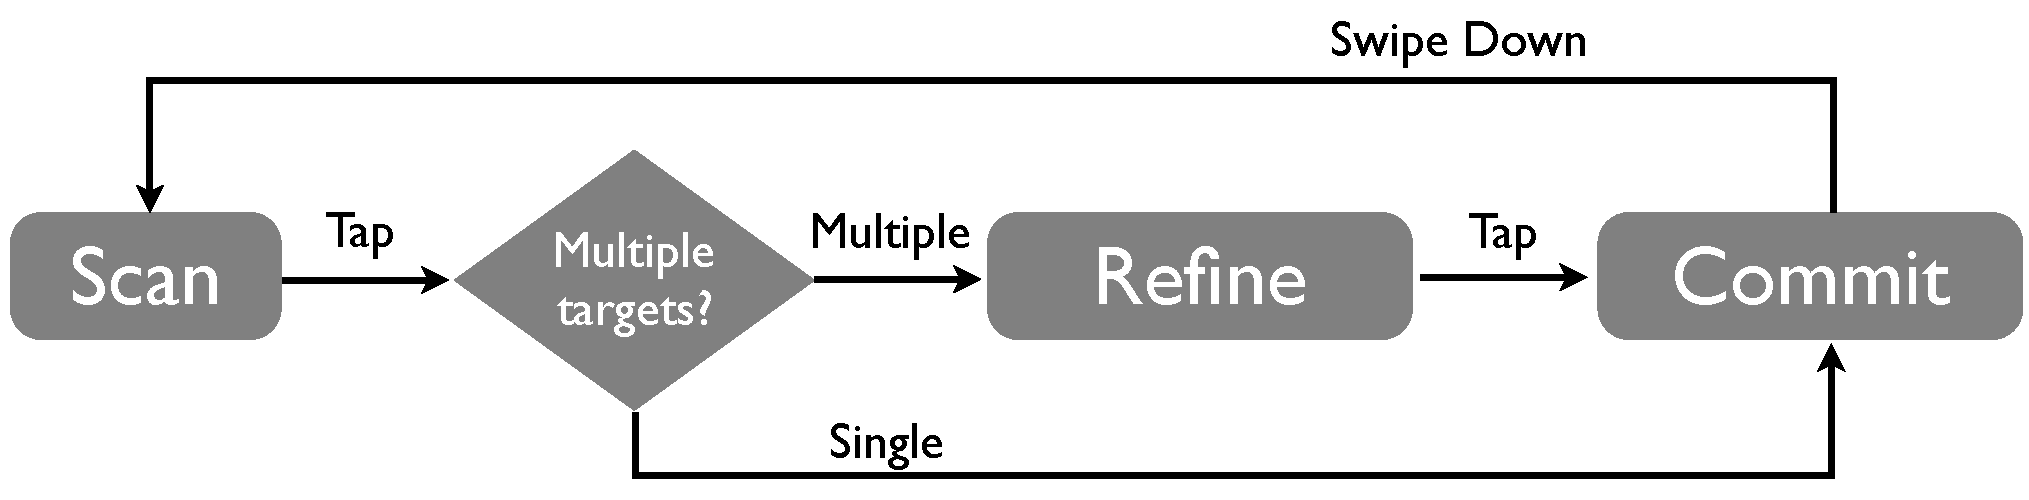
\includegraphics[width=\columnwidth]{figures/interactionModel2.pdf}
\caption{{\em scan} and {\em refine} -- two main stages during the interaction with HOBS. For completeness, we have also added the final state of {\em commit}.} 
\label{fig:interaction}
\end{figure}

The overall target acquisition time thus depends on scan and refine times, the probability that refinement is needed, and the time to commit an action (tap):
\begin{equation}
t_{total}=t_{scan}+P(refine)*t_{refine}+t_{commit}
\label{eq:time}
\end{equation}

In the following sections, we describe our iterative design and evaluation process to minimize the overall target selection time.

%%% Local Variables: 
%%% mode: latex
%%% TeX-master: "uist14"
%%% End: 



\section{Hardware Device}
\begin{figure}[t]
\centering
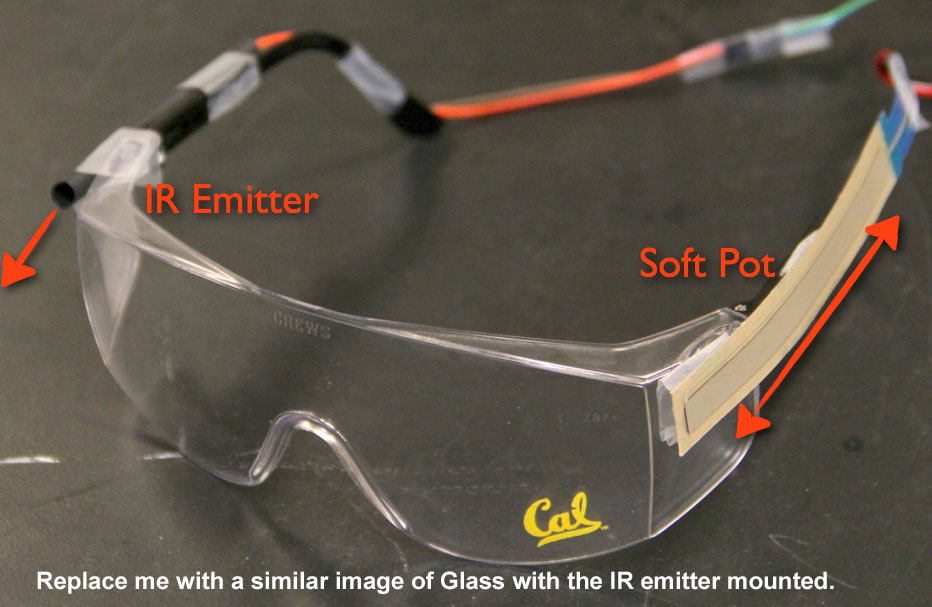
\includegraphics[width=1.0\columnwidth]{figures/glass-with-ir}
\caption{Our augmented Glass prototype has a frame-mounted infrared emitter.}
\label{fig:glass}
\end{figure}
\begin{figure}[t]
\centering
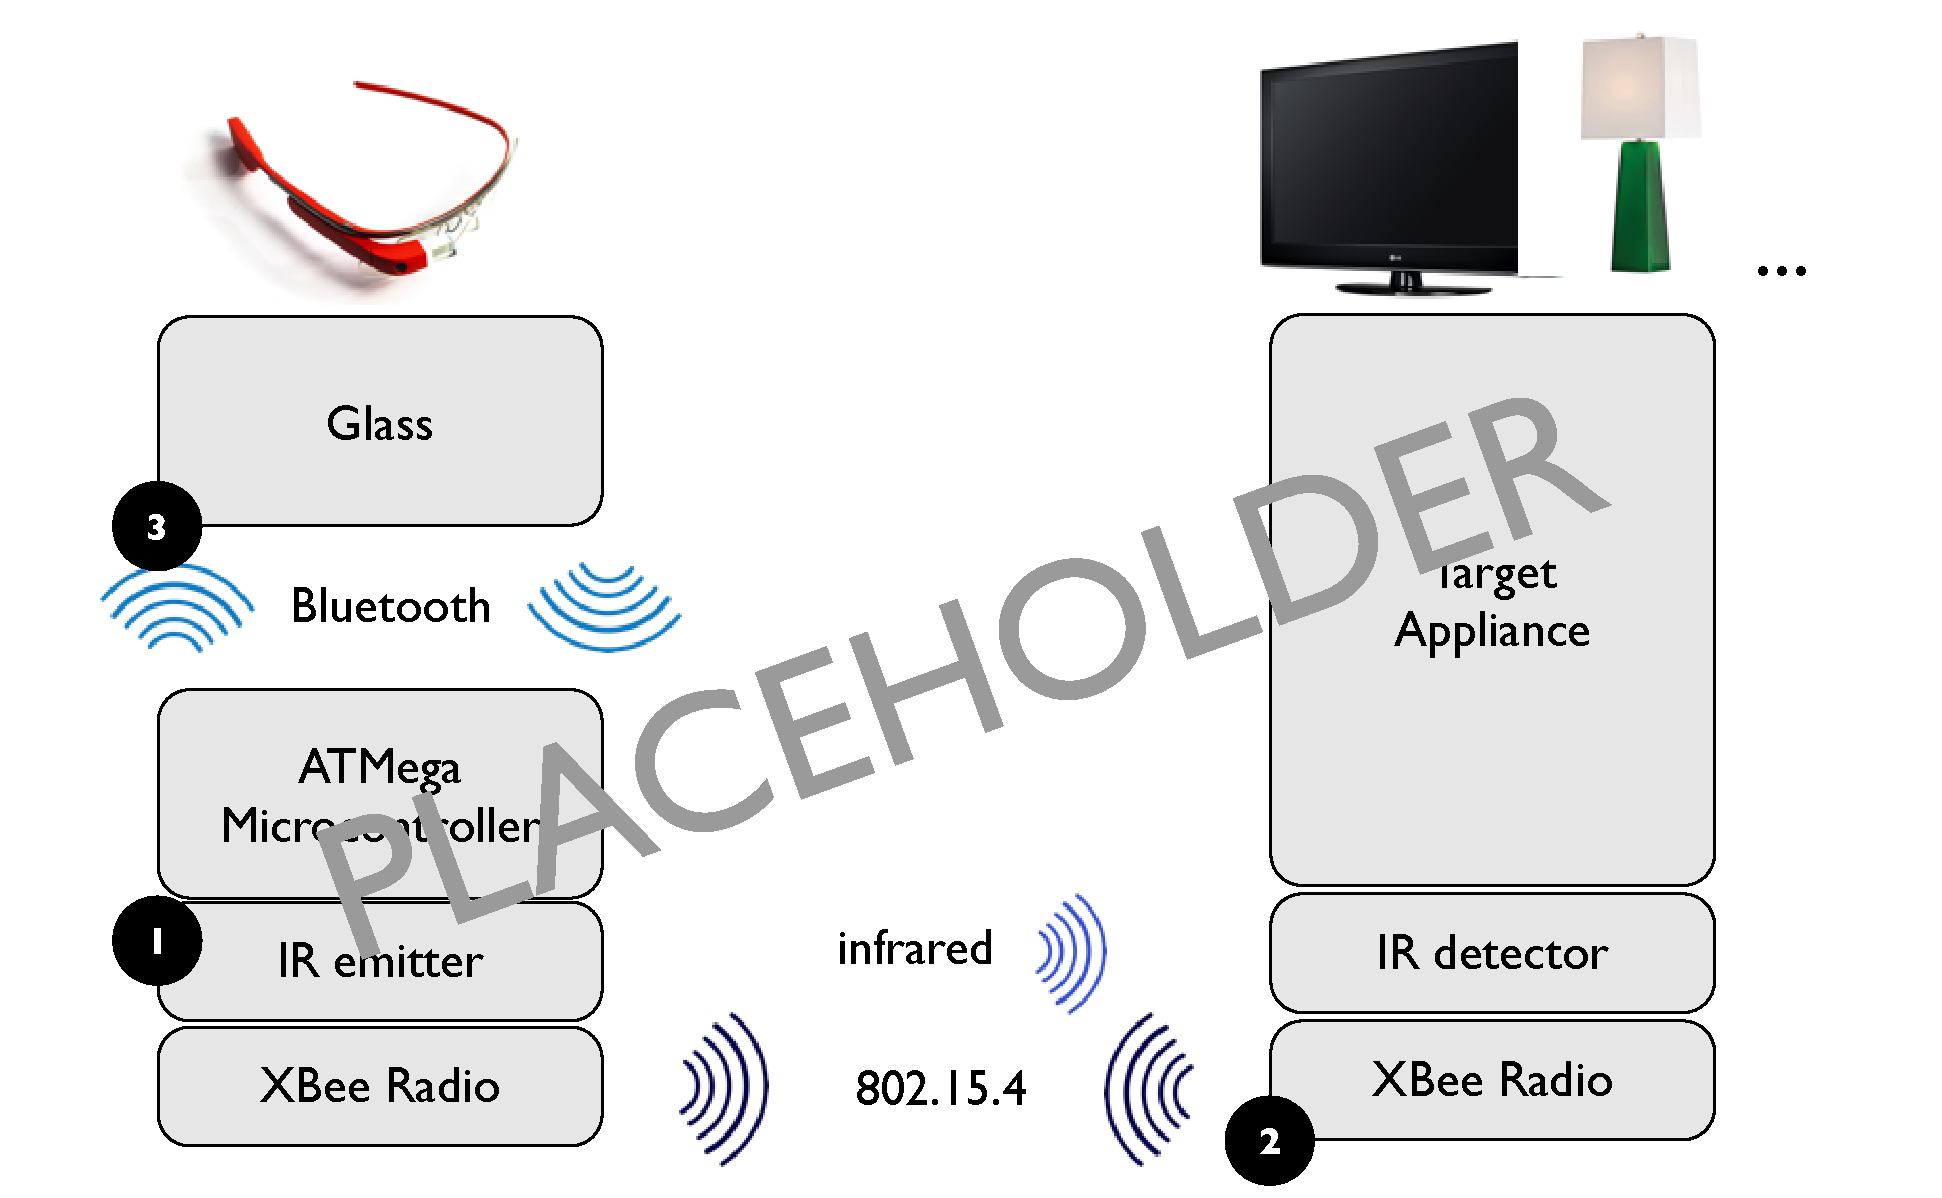
\includegraphics[width=1.0\columnwidth]{figures/architecture}
\caption{In our system architecture, selection is initiated through infrared but confirmed over 802.15.4. This permits wearers to move their head freely after connecting to an appliance. In the research prototype, users have to carry an additional microcontroller board that marshals messages between Glass' Bluetooth radio an IR/802.15.4, but our custom hardware could also be integrated into the wearable device.}
\label{fig:architecture}
\end{figure}

\subsection{Prototype Implementation}
Our prototype consists of a Google Glass Explorer Edition head-worn computing device, augmented with an infrared emitter that is mounted on the frame, pointing out in the direction of the wearer's view (Figure~\ref{fig:glass}). The IR emitter LED is mounted in an opaque hollow tube, that restricts the outgoing angle of illumination. 

In our prototype, Glass communicates over Bluetooth to an additional microcontroller board the user has to wear (Atmel ATMega256). This board marshals XBee to Bluetooth messages in both directions and also controls the IR LED mounted on the Glass frame (Figure~\ref{fig:architecture}). This architecture was mostly chosen for reasons of expediency. We selected XBee 802.15.4 radios to avoid Bluetooth  wake up latencies but we do not claim optimality for our design decisions. Future head-mounted devices could clearly integrate IR emitters; the choice of local wireless technology could also change. In particular, one could substitute WiFi modules or design an all-Bluetooth network.

\afterpage{
\begin{figure}[t!]
\centering
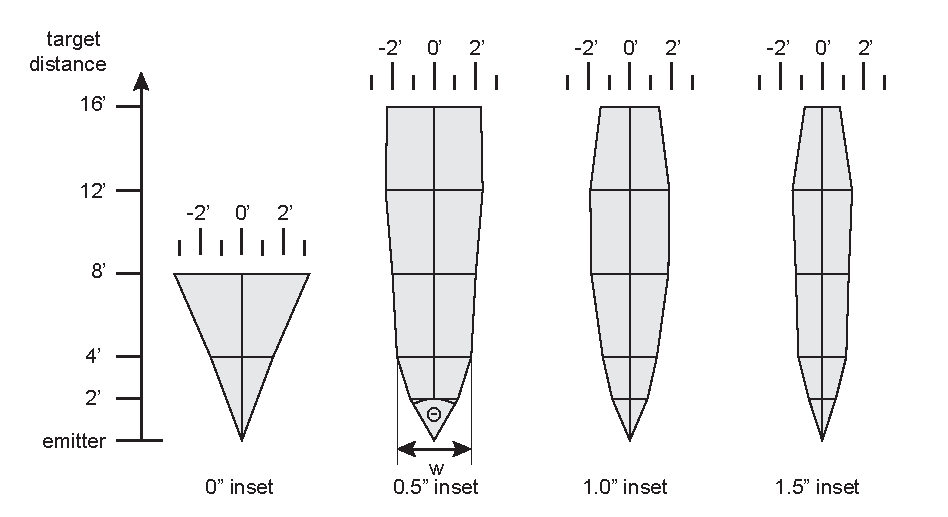
\includegraphics[width=1.0\columnwidth]{figures/glass-ir-coverage}
\caption{Different IR configurations suggest usable beam widths of 2 to 4 feet and distances up to 16 feet }
\label{fig:coverage}
\end{figure}
\begin{table}[h!]
    \begin{tabular}{l|lllll}
    distance/ depth & \ft2       & \ft4       & \ft8   & \ft{12}  & \ft{16}  \\ \hline
    \inch{0}                     & $74\degree$ & $78\degree$ & N/A  & N/A  & N/A  \\
  \inch{0.5}                   & $60\degree$ & $48\degree$     & $28\degree$ & $22\degree$ & $16\degree$ \\
    \inch{1.0}                     & $46\degree$     & $36\degree$     & $26\degree$ & $18\degree$ & $10\degree$ \\
    \inch{1.5}                   & $36\degree$     & $32\degree$     & $18\degree$ & $14\degree$ & $6\degree$  \\
    \end{tabular}
    \caption{Measured IR coverage angles $\Theta$ at different target distances and different depths of IR emitter inside shielding tube.}
    \label{table:measurements}
\end{table}
} %end afterpage

\subsection{Device Characterization}
We determined the usable range and accuracy empirically with one IR emitter and two IR receivers. The IR emitter constantly sent out an id signal. The receivers that correctly received the signal turn their LED on for 300 ms.

We placed all three devices at the same height with clear line of sight. The IR emitter is first places 2 feet away from the receivers. The receivers were moved sideways apart from each other until they could no longer receive stable signals. We then recorded the distance of the two receivers for the calculation of coverage angles. The steps are repeated for IR emitters in different distances (as shown in Table~\ref{table:measurements}). We then repeated measurements with the emitter  placed at various depths in the tube (see Figure~\ref{fig:coverage}). 

In summary, our measurements suggest that IR communication can be targeted to an area about 2--4' in diameter, up to 16' in front of the user. These values are a reasonable match for selecting appliances in a room-size environment. A wider beam would lead to an increased chance of multiple appliances receiving IR signals simultaneously. A narrower beam will make targeting more challenging, given the precision constraints of human head movement.


\section{Physical Target Acquisition Study}
To understand the accuracy and performance of head-orientation-based  selection through our device, we carried out a comparative target acquisition study, where participants had to connect to wireless nodes distributed in a room with our technique, and with an alternate list selection approach.

\begin{figure}[t]
\centering
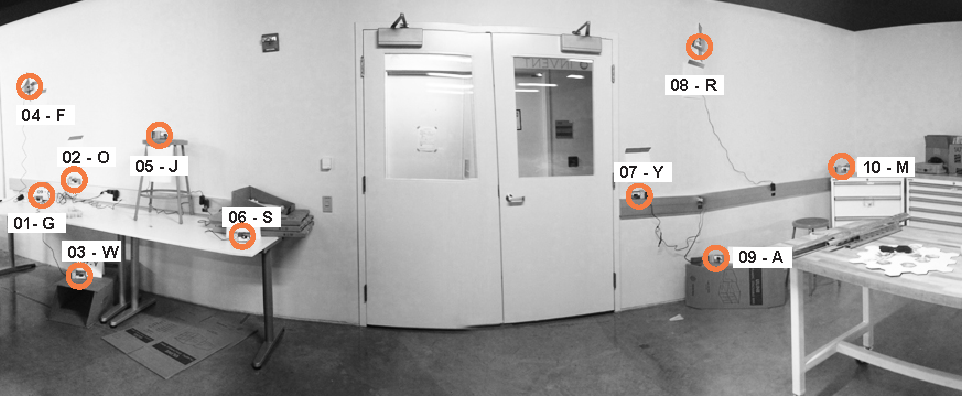
\includegraphics[width=1.0\columnwidth]{figures/targeting-study-layout.pdf}
\caption{In the targeting study, participants had to find and select one of 10 targets in a lab environment.}
\label{fig:targeting-study-layout}
\end{figure}

\subsection{Apparatus}
In an indoor environment, 10 wireless nodes are spread across a room at various heights and distances (see Figure~\ref{fig:targeting-study-layout}). The nodes are stand-ins for potential smart appliances and have all relevant functionality for targeting and wireless communication, but do not control any actual appliances. Each node is an embedded wireless system with a microcontroller, IR receiver, a wireless XBee radio, and three status LEDs (see Figure~\ref{fig:target}). An orange LED indicates that the device is the target that should be selected in the current trial; a red LED lights up whenever the device receives an IR signal from Glass; a blue LED shows when participants have successfully connected to a device, and is also used for disambiguation when multiple clients are within IR range . Next to each client device, a paper sheet shows a number and letter combination, which are used for uniquely identifying the devices. \sean{The numbers are the primary identifiers while the letters are in raondom order. The nodes are somewhat sorted by their numbers, making it easy to find in order to simulate a place the users are more familiar with. Therefore, the time spent on finding the target was minimized and the time measured was mainly the acqusition time. }


\begin{figure}[b]
\centering
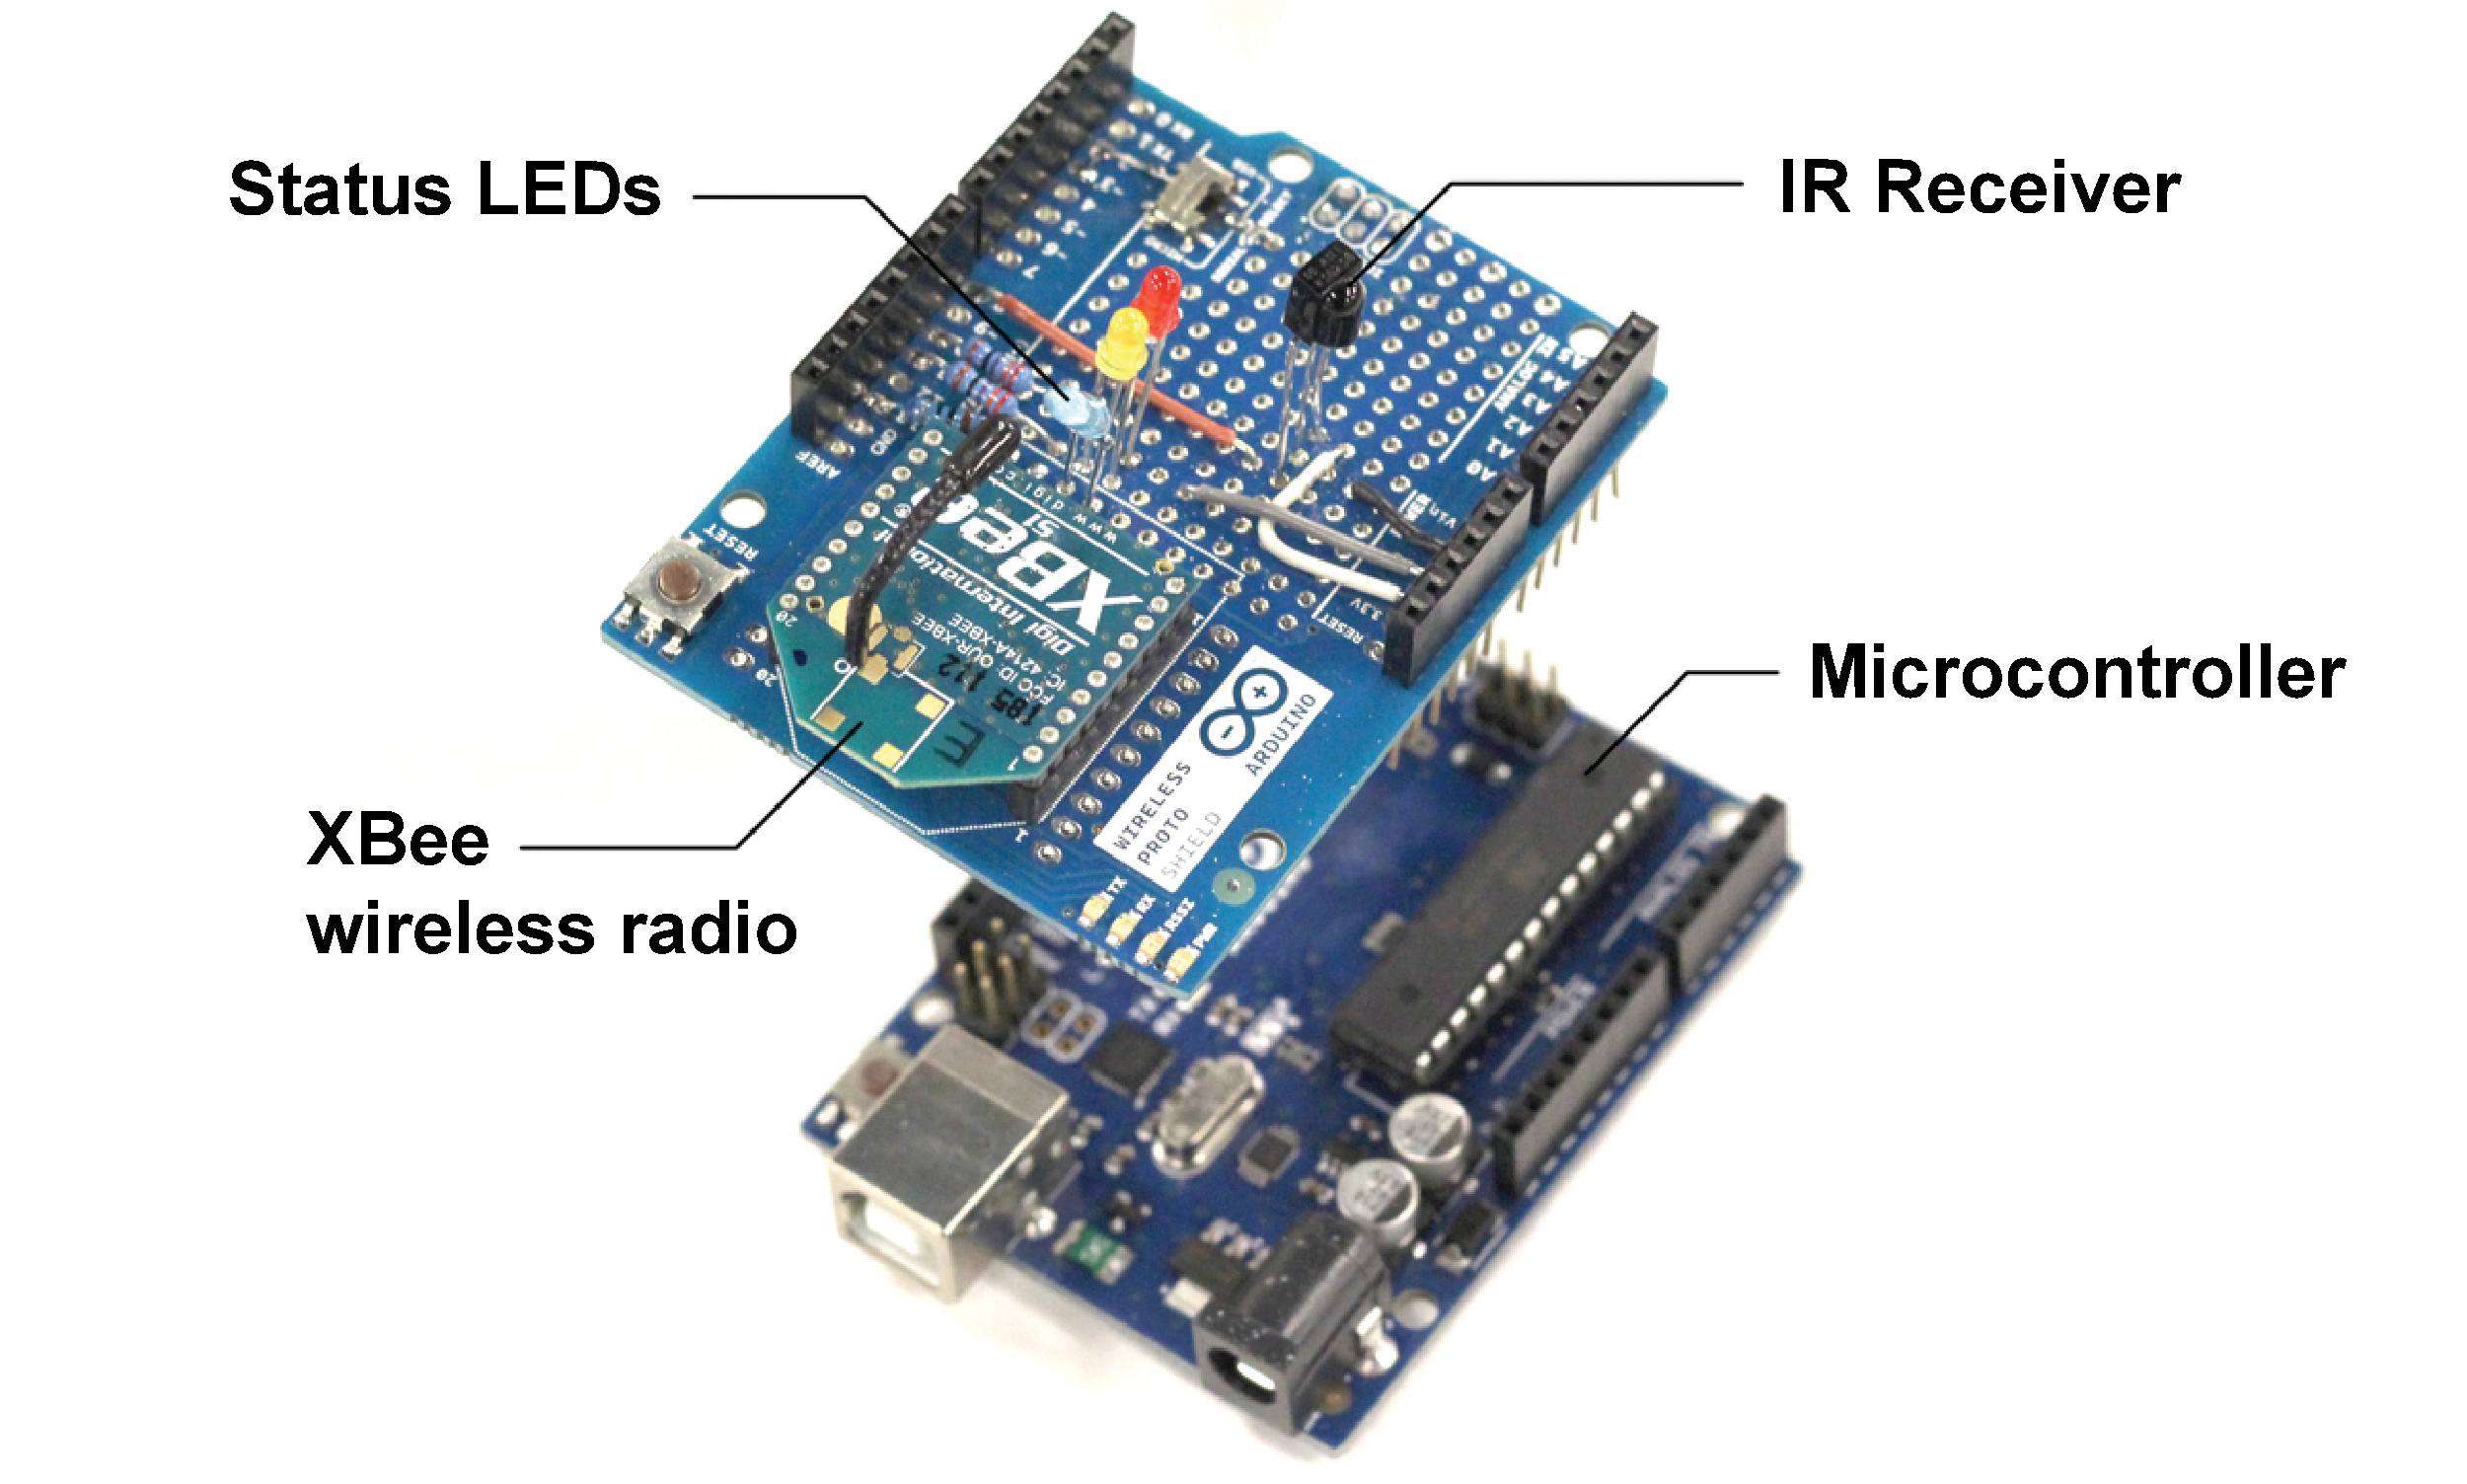
\includegraphics[width=0.8\columnwidth]{figures/study-node.pdf}
\caption{An example node from the targeting study --- we constructed 10 such nodes - each mounted in a box.}
\label{fig:targeting-study-layout}
\end{figure}

\subsection{Methodology}
In our within-subjects design, participants performed 15 target acquisition tasks each with two interaction styles. In the {\em infrared} condition, participants used our IR targeting approach; in the {\em list} condition, participants had to look up a device's letter code on the printed paper next to the device and then select that letter code from a list displayed on their Glass device. The list was navigated with swipe motions on the Glass touchpad. For each task, participants started at a fixed position in the room. The experimenter called out a number and simultaneously started a timer. Participants then had to find the corresponding device (by looking for its printed code). In the {\em infrared} condition, participants then selected and acquired the target by aiming the infrared beam at the target, and confirmed their selection with a touch pad tap. If more than one target was within range, participants had to either use the disambiguation dialog or reposition themselves. In the {\em list} condition, participants had to read the letter next to the number and then select that letter by browsing a linear list shown in their Glass display. While the list was alphabetized, letter arrangement in the room was not. This design required participants to find the target in the room before starting a list navigation to keep conditions similar to each other.

Afterwards, participants completed a survey that elicited answers to Likert-scale questions as well as open-ended answers about their experience.

\subsection{Participants}
We recruited \bjoern{N} participants from our institution. \bjoern{X} had never used Glass before. \bjoern{Y} wore prescription glasses, which may have affected their task performance as wearing both Glass and regular glasses is possible, but leads to \bjoern{explain problems}.

\subsection{Measures}
The main measures were {\bf target acquisition time}: the time required to identify, select, and connect to a wireless target device; and {\bf user preference}: which interface users preferred for the task after completing the study.

\subsection{Results}
\subsubsection{Performance data}
The time to complete each task can be broken down into the following pieces:

$t_{infrared}=t_{locate}+t_{reorient}+t_{disambiguate}+t_{tap}$

$t_{list}=t_{locate}+t_{listnav}+t_{tap}$

In both conditions, participants first have to locate the target announced by the experimenter ($t_{locate}$). In the {\em infrared} condition, participants may then directly confirm their selection if only a single target was selected ($t_{tap}$). However, if they don't immediately receive feedback that their target was selected, or if multiple targets were selected, users either have change their position or head orientation ($t_{reorient}$) or they have to step through the on-screen disambiguation dialog ($t_{disambiguate}$). In the {\em list} condition, participants must scroll through the list to find the desired target identifier ($t_{listnav}$).
This analysis makes it clear that any performance benefit depends on whether $t_{reorient}+t_{disambiguate}<t_{listnav}$. This depends on the number of total devices in the environment (increasing $t_{listnav}$), and their density (which will increase $t_{disambiguate}$). 

At 10 devices, total selection times are comparable:
\bjoern{Hopefully, when adding distractors, the list navigation will become very cumbersome.}

\begin{figure}[t]
\centering
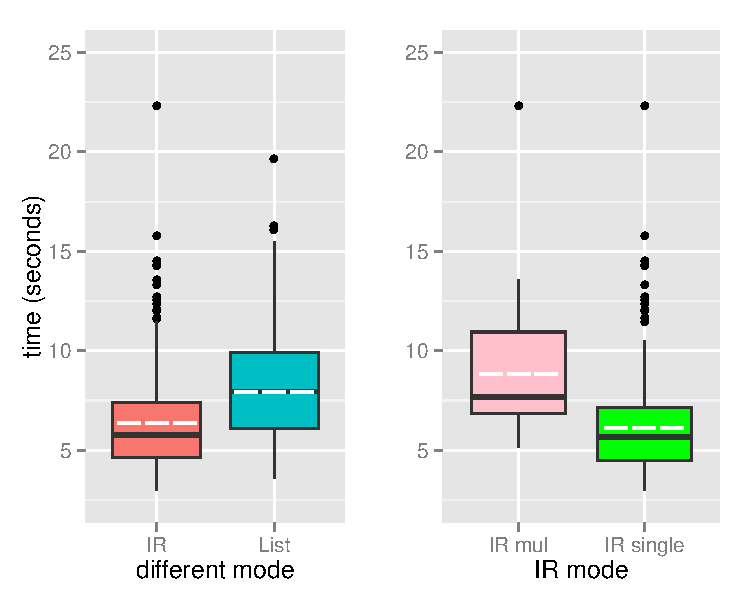
\includegraphics[width=1.0\columnwidth]{figures/R_time_by_Category.pdf}
\caption{Task completion times.} \sean{label mean on the chart}
\label{fig:selection-times}
\end{figure}

As a result, infrared mode out performs list mode by 2.186 seconds (6.672 vs 8.858), as shown in figure~\ref{fig:selection-times}. \sean{TBC}  

\begin{figure}[t]
\centering
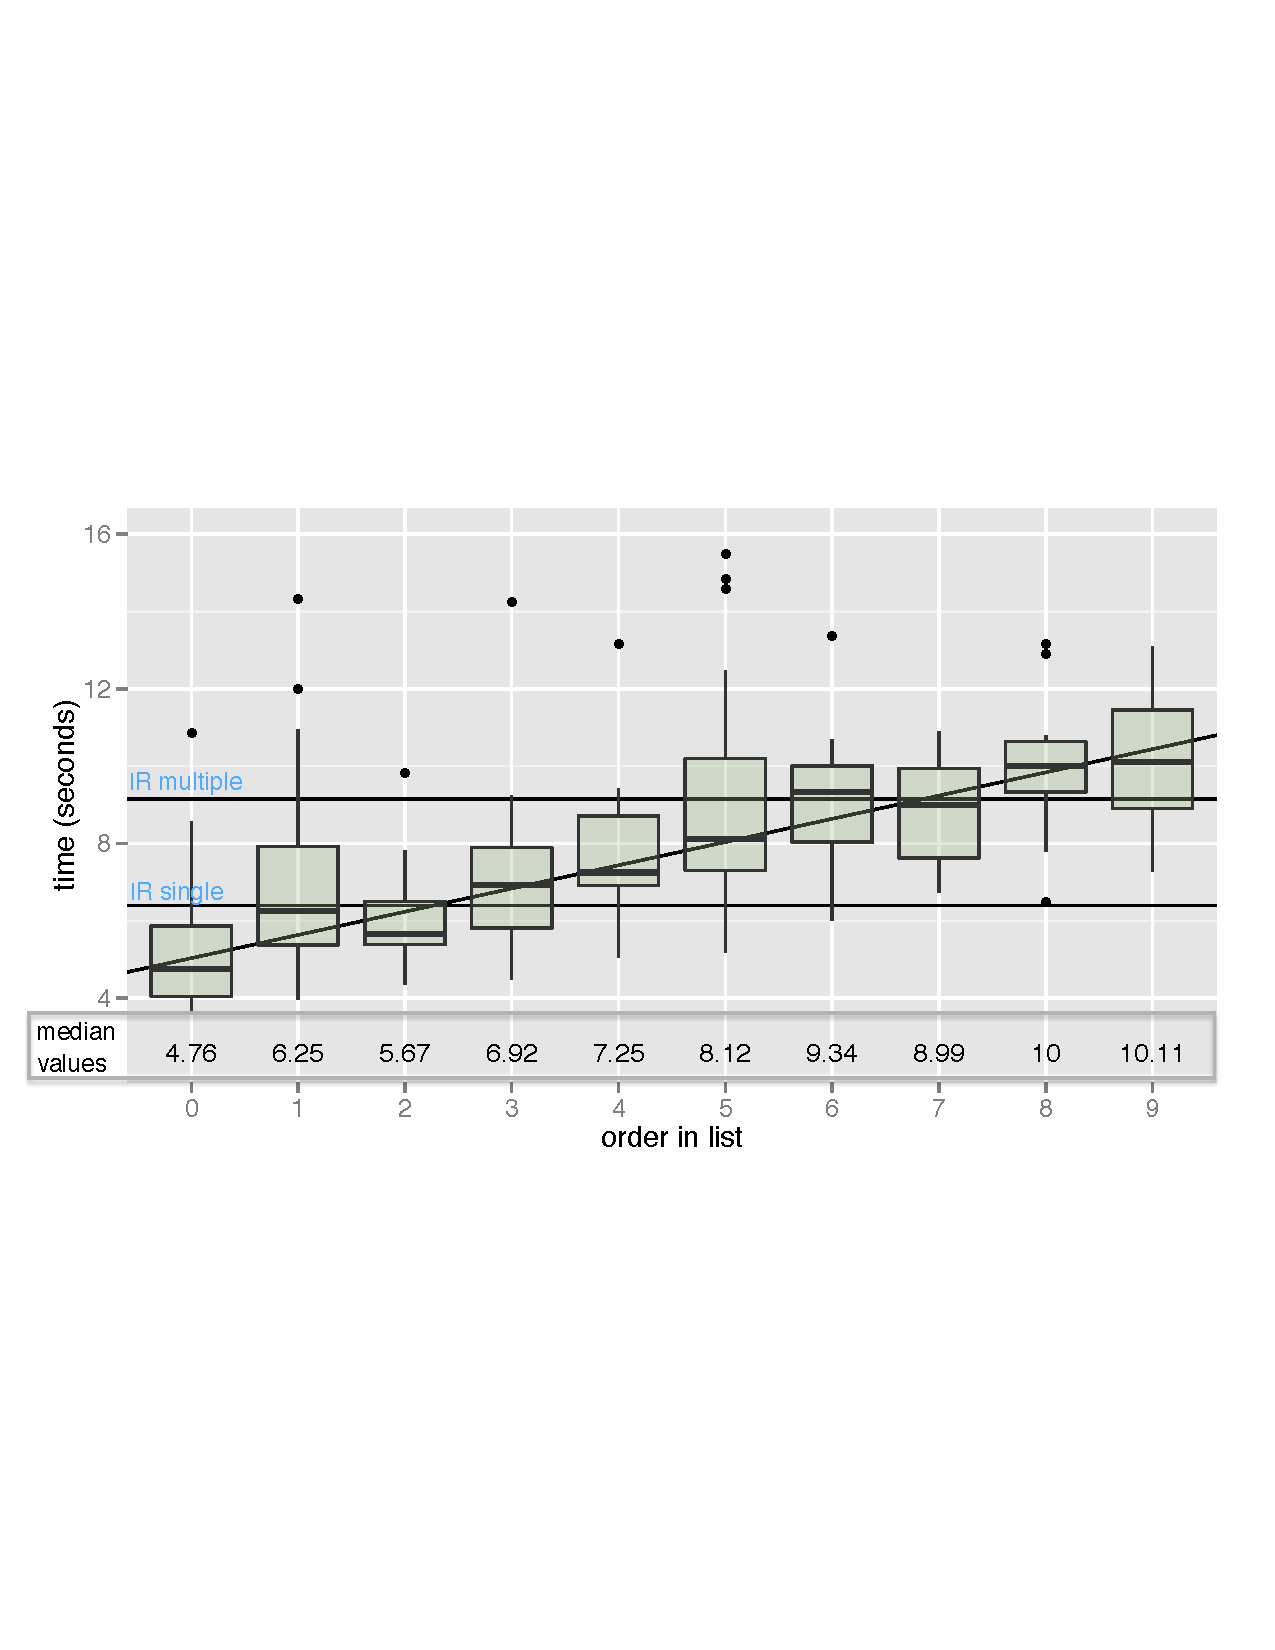
\includegraphics[width=1.0\columnwidth]{figures/R_List_by_Target.pdf}
\caption{Average time taken vs. the order of nodes on the list }
\label{fig:time-vs-list-order}
\end{figure}


\begin{figure}[t]
\centering
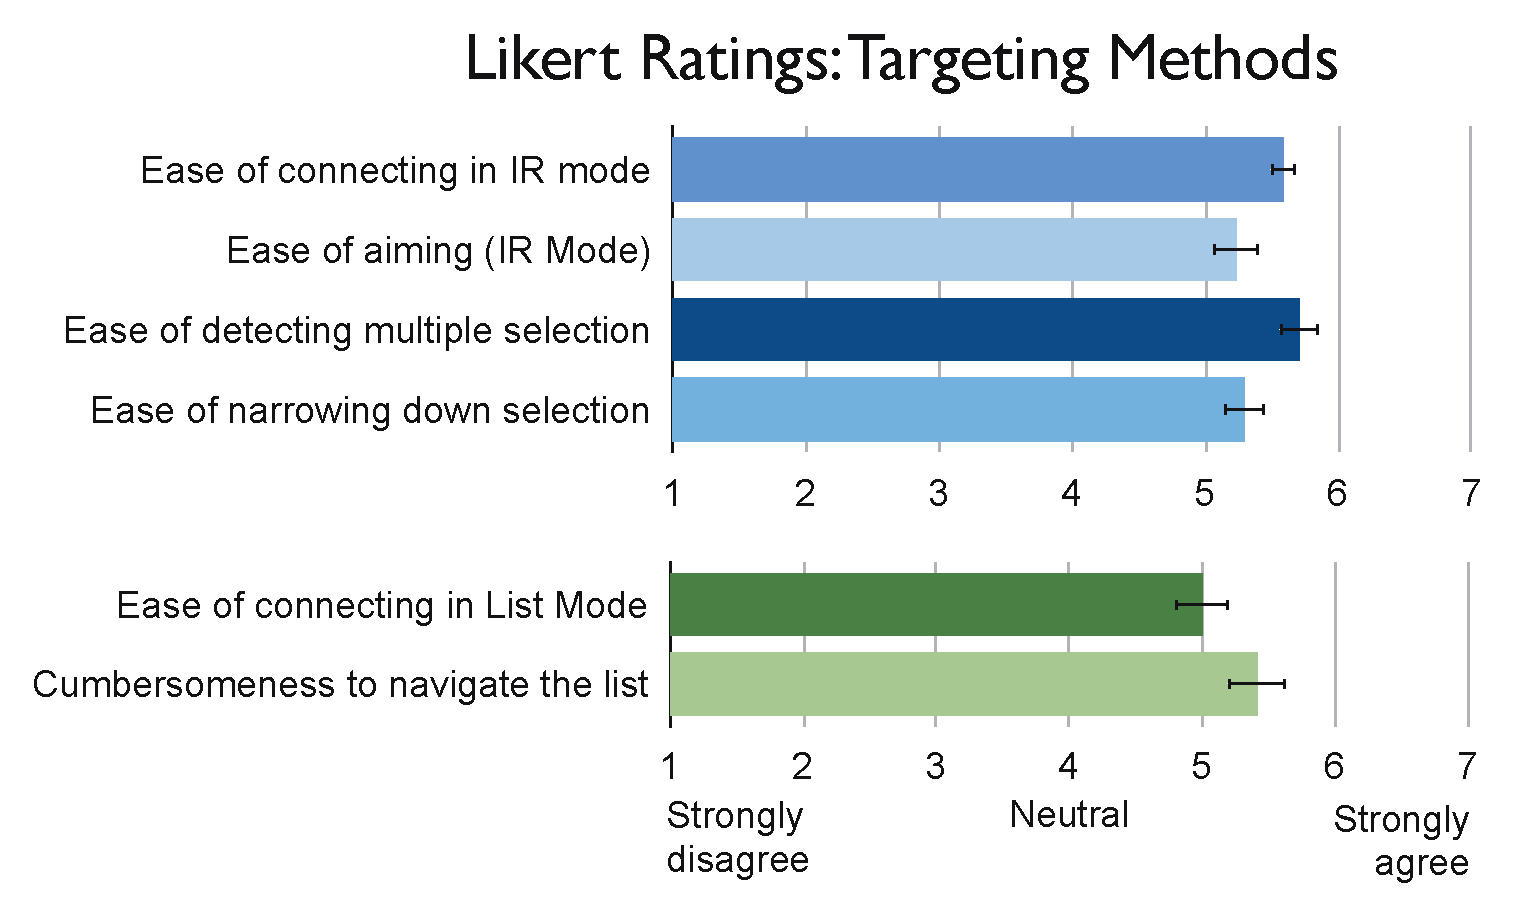
\includegraphics[width=1.0\columnwidth]{figures/target-likert.pdf}
\caption{Likert scale ratings for ease of use of aspects of the targeting task. Error bars show standard error. }
\label{fig:target-likert}
\end{figure}

\subsubsection{Preference}
\bjoern{update: 6 of 7} users preferred infrared mode over list mode. While both interfaces were judged similarly on overall ease of connecting, list navigation received the lowest likert scores (see Figure~\ref{fig:target-likert}). As self-report data can easily skew positive as participants try to please experimenters, we also asked participants to elucidate why they preferred one interface over the other.

List mode had certain advantages: It was judged to be more accurate and predictable as there was always exactly one device selected in the list (\studyquote{With the list you never have to worry about accidentally picking up two targets}). Also, it did not require a clear line of sight to the target device so participants did not have to move from their starting position (\studyquote{The shortcoming of the IR mode was that you had to be a certain distance away in order for it to detect the appliance}). 

On the other hand, list mode was judged to be more \studyquote{annoying} and tedious. The temple-based touchpad for selection was difficult to use for a participant with long hair: \studyquote{List mode was physically difficult for me to navigate, since my long hair wasn't tied back and it kept interfering with my swiping.} Another participant also commented on the ergonomic challenge of touchpad use on Glass: \studyquote{The strength of the IR mode was that I didn't have to use my fingers as much to control. If the items were spaced relatively far apart, it was easy to select a specific appliance.}

\bjoern{add more from survey answers}.

%IR mode has semantic meaning (like I said).  I'm likely to want visual feedback from any distant device I'm trying to control, and since I'm already looking at it, this is very easy to get.  List mode was physically difficult for me to navigate, since my long hair wasn't tied back and it kept interfering with my swiping.  Another comment about list mode was that swiping faster didn't seem to navigate the list faster, which would have been convenient for accessing items like W and Y very far from the beginning of the list.  This could also be partially overcome by using a circular linked list (where the list wraps from Y to A) instead of a one-way list.
%With the list you never have to worry about accidentally picking up two targets, but since you always have to swipe through a (longer) list that's not much of an advantage.
%List mode felt like I could be more confident in what client I was choosing because I couldn't select more than one client. The IR mode was a little more natural because it involved less clicking and navigating, but it felt easier to select the wrong client which made the list mode more comfortable. 
%"The shortcoming of the List mode was that the list didn't wrap around. So for example if I wanted to go to Y, I couldn't just go left from A—I had to scroll through all the letters in between.

%The strength of the list mode was that it's pretty accurate, so as long as I swiped the correct amount, I could activate and power off the appliances. I also didn't have to move at all, although perhaps that is a shortcoming because otherwise we might just all turn into Wall-E people.

%The strength of the IR mode was that I didn't have to use my fingers as much to control. If the items were spaced relatively far apart, it was easy to select a specific appliance. 

%The shortcoming of the IR mode was that you had to be a certain distance away in order for it to detect the appliance. "
%The List Mode is easier to choose the desired item when the item list is short. It became a bit frustrated when I had to swipe many times in order to get to the targeted item. The IR mode works more intuitive in this case, but need a longer time to learn and get used to it.
%list mode is easier to select what you want, but may take a while to get to since you can only swipe through one at a time; IR is quicker and more intuitive, but unstable
%"list mode is annoying. i find myself counting how many swipes i have to do.

%IR mode is fun and pretty convenient"



\section{Example SmartHome Scenario}
To understand how our device could be used to interact with smart appliances, we also asked all study participants to work through a concrete scenario. The main goal was to obtain qualitative feedback on the usability and utility of our device with more realistic tasks.

\begin{figure}[t]
\centering
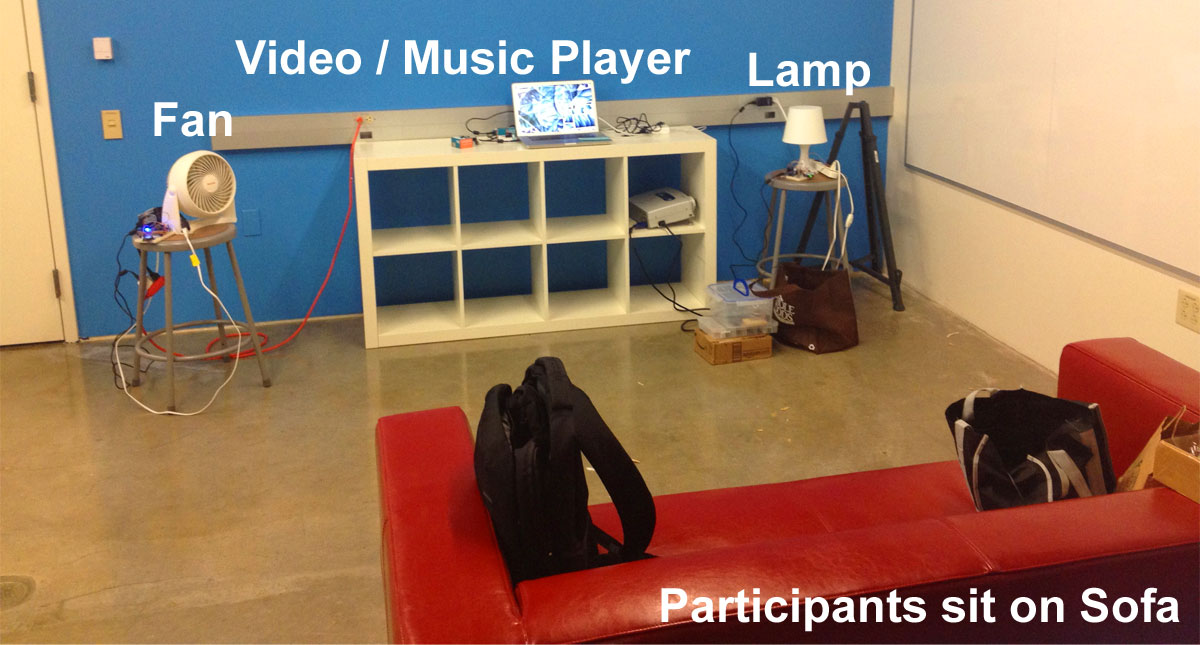
\includegraphics[width=1.0\columnwidth]{figures/smarthome-scenario.jpg}
\caption{In the smart home scenario, participants completed a series of appliance control tasks in a simulated living room.}
\label{fig:smarthome}
\end{figure}

\subsection{Methodology}
We recreated a living room environment that had four controllable appliances: a fan, a lamp, and two laptops functioning as an audio and video player, respectively (see Figure~\ref{fig:smarthome}). The fan and lamp had binary controls: they could be switched on or off. The laptops had multiple parameterized functions: participants could start, pause, stop, and rewind  video and audio, and adjust volume.

We then asked users to work through the following script for controlling the room for watching a movie in the evening:
{\small
\begin{enumerate}
\item Turn off the lights as you want to watch the movie in a darkened room.
\item You feel a little hot in the room, so you turn on the fan.
\item You connect to the Smart TV and start playing the movie. 
\item The volume seems too soft to hear over the fan- turn it up a bit. 
\item After a while, you want to take a break to get a snack. Pause the movie. 
\item When you come back, you've forgotten what was said last - rewind by ~30 seconds and restart the movie. 
\item When the credits roll, you stop the movie and turn the lights back on.
\item You want to listen to some music.
\item After awhile, you stop the music you turn off the fan and leave the room.
\end{enumerate}
}

For this study, we only elicited subjective data in the form of Likert data and 
\begin{figure}[b]
\centering
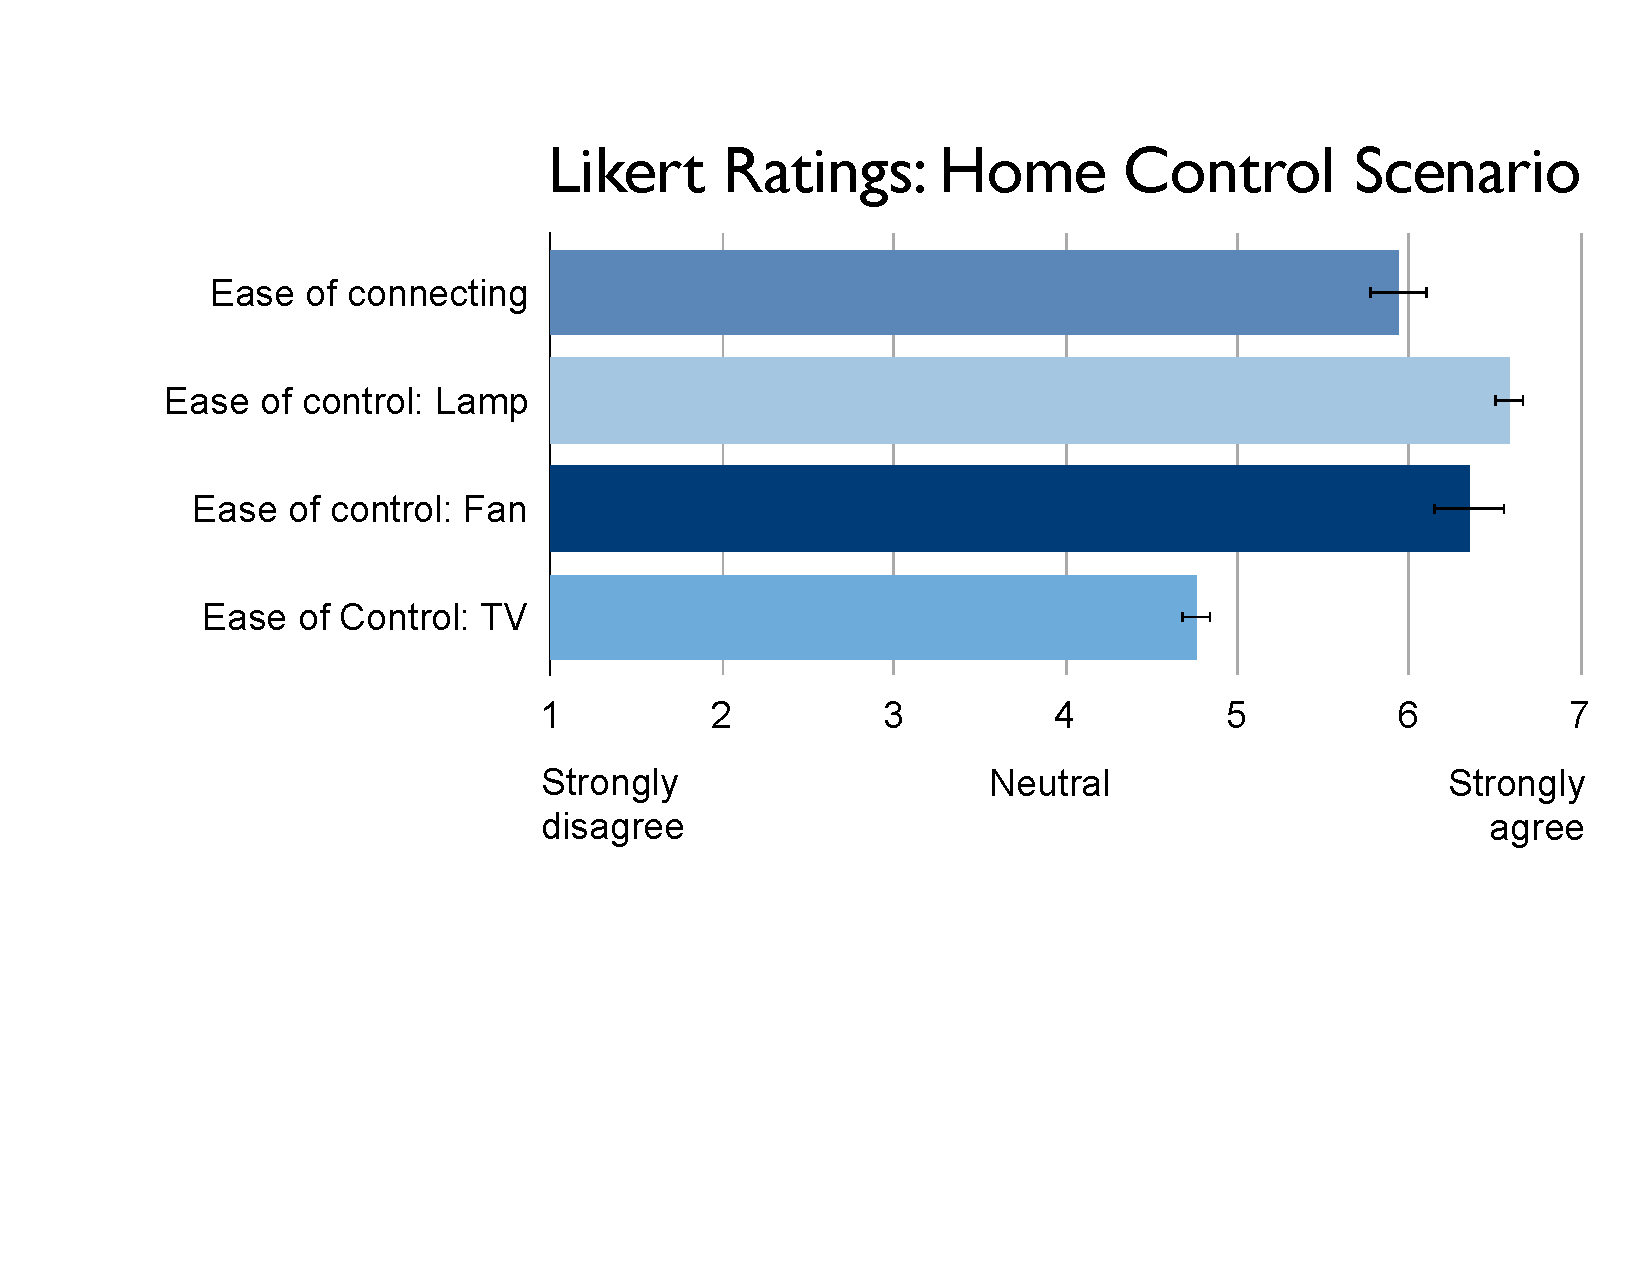
\includegraphics[width=1.0\columnwidth]{figures/scenario-likert.pdf}
\caption{Likert scale ratings for ease of use of aspects of the smart home control scenario. Error bars show standard error.}
\label{fig:smarthome-likert}
\end{figure}

\subsection{Results}
All participants successfully completed the list of tasks.
Participants stated it \studyquote{felt easy to interact with the appliances}, but there were distinct differences between appliances. Ease of use ratings were higher for the lamp and fan which had simple, discrete on/off actions, and lower for more complex TV and music player devices (see Figure~\ref{fig:smarthome-likert}). Multiple participants remarked that the difficulty was based on the affordances of Glass: \studyquote{Most of the difficulty I had with Glass came from having to navigate the interface on the tiny screen with the touch pad}. The screen size and 1D input thus likely put a limit on the complexity of interfaces that can be presented.

\bjoern{explain why music is so low, if this trend holds}

\subsubsection{Visual overlap between Near-Eye Display and Target Appliance}
When a participant looks at a target, the near-eye display may occlude or overlap the target appliance. This may make it difficult to read either the on-screen display or see information displayed on the target device.  As one participant remarked \studyquote{This was especially annoying with the TV because there were two screens overlapping each other.} While it is possible to look away once a device has been acquired to better see the Glass display, this tension is likely to remain for users who want to rely on feedback from the devices themselves instead of the Glass display.

\subsubsection{Control}

%Overall it felt easy to interact with the appliances. I imagine that moving backwards and forwards in the video by swiping could get frustrating if one were trying to move by just a little bit, or to a specific spot."
%Operating the lamp and fan felt very natural because each only involved turning it on or off, which can be done with tapping Glass once. Most of the difficulty I had with Glass came from having to navigate the interface on the tiny screen with the touch pad, but only clicking once made use a lot easier. The TV was a little more difficult to operate because there were more options on the display. Tapping felt more natural than the multi-touch gestures.
%"Again, the lack of movement is both good and bad. It's good in that you can just stay in one place and control everything.  Also, everything is centralized, so you don't need to use multiple switches. I liked the two-finger touch to change the volume as well as to fast-forward/rewind. It's clever.  The only issue with it, though, was that I felt like I didn't have as fine-grained control, but perhaps that's because I have not practiced swiping with Glass much.

%I didn't like that it promotes a sedentary lifestyle. Also, I disliked how it took away the tactile feeling that you get from pushing buttons. I didn't like how you had to scroll through a bunch of things to access certain items when otherwise I could just have flipped a switch."
%I think it's cool to control home appliances by using Glass if the home devices are far from the place where the user is. It might also be useful for people who need to take care of small children that they can complete all the tasks while keeping an eye on their children at the same time.
%it was easy to connect, but it was annoying to have to first connect to turn on/off - I kept trying to point and then immediately click to turn on/off, but I had to do the extra step of connecting THEN turning on/off.  I also tried to point back at the appliance when I was already connected.  I intuitively want the screen to automatically appear when the IR detects the appliance rather than having to tap to connect.
%"i liked the feeling i had while doing the selection etc

%i disliked that lag time where i was looking at the thing i wanted to control and it wasn't responding to me - about 500ms or so of interaction discomfort"


\section{Discussion}
\label{sec:discussion}

We discuss a few issues with the system.
%%% Local Variables: 
%%% mode: latex
%%% TeX-master: "uist14"
%%% End: 

\section{Conclusion}
We introduced a novel method for selecting and controlling smart appliances in physical spaces through  infrared targeting based on head orientation. The design takes advantage of the fact that visual attention can express intention, makes it ituitive and helps users remain their focus in the physical world. It addresses the naming and scaling challenges faced by handheld mobile devices. While we present a prototype approach that requires that the user carry additional hardware, all parts can readily be miniaturized and integrated into future head-worn hardware. We also introduced a disambiguation technique in case head orientation is not sufficient to determine a unique target. We characterized our devices performance, arguing that it is matched well to the amount of head movement people can control without strain. A target acquisition study showed that the technique is efficient; a home control scenario showed promise but also limitations when trying to control complex appliances. As our environment continues to be populated by a swarm of sensing and actuation devices, methods to interrogate and control our smart environments may become increasingly important.
%\section{Acknowledgments}
%We thank our user study participants and the a

%figure template:
%\begin{figure}[!h]
%\centering
%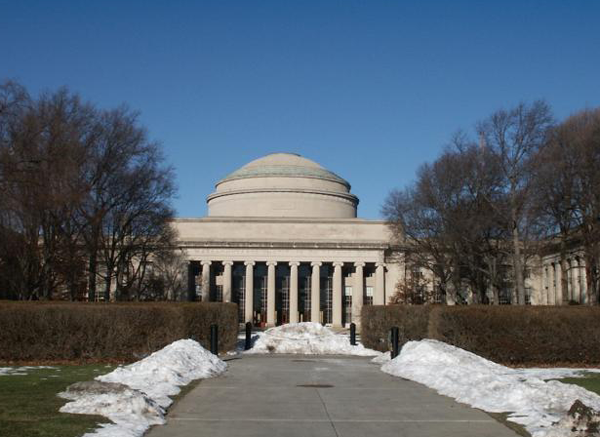
\includegraphics[width=1.0\columnwidth]{Figure1}
%\caption{With Caption Below, be sure to have a good resolution image
%  (see item D within the preparation instructions).}
%\label{fig:figure1}
%\end{figure}


% Balancing columns in a ref list is a bit of a pain because you
% either use a hack like flushend or balance, or manually insert
% a column break.  http://www.tex.ac.uk/cgi-bin/texfaq2html?label=balance
% multicols doesn't work because we're already in two-column mode,
% and flushend isn't awesome, so I choose balance.  See this
% for more info: http://cs.brown.edu/system/software/latex/doc/balance.pdf
%
% Note that in a perfect world balance wants to be in the first
% column of the last page.
%
% If balance doesn't work for you, you can remove that and
% hard-code a column break into the bbl file right before you
% submit:
%
% http://stackoverflow.com/questions/2149854/how-to-manually-equalize-columns-
% in-an-ieee-paper-if-using-bibtex
%
% Or, just remove \balance and give up on balancing the last page.
%
\balance

% REFERENCES FORMAT
% References must be the same font size as other body text.

\bibliographystyle{acm-sigchi}
\bibliography{sigchi14}
\end{document}
